\section{Footstep Evaluation Network}
\label{sec:methodology-footstep-evaluation-network}

The purpose of the footstep evaluation network is to generate
footstep candidates for the GaitNet model. Importantly, the precise
output of this network is not critical; rather, it is essential that
the network provides high-quality candidates when sampled. It
achieves this by estimating the cost associated with potential
footsteps given the current robot state. The network’s architecture
and training process are largely based on ContactNet
\cite{bratta_contactnet_2024}, with several key modifications, which
are described in detail below.

%%%%%%%%%%%%%%%%%%%%%%%%%%%%%%%%%%%%%%%%%%%%%%%%%%%%%%%%%%%%%%%%%%%%%%%%%%%%%%%%
\subsection{Architecture}
\label{subsec:methodology-contactnet-architecture}

The footstep evaluation network is responsible for generating a set
of footstep candidates $\mathbf{f_c}$ based on the robot state $\mathbf{x_c}$:

\[
  \mathbf{x_c} =
  \begin{bmatrix}
    \mathbf p_{b,xy} \\
    \mathbf r_{w,z} \\
    \mathbf v_b \\
    \mathbf \omega_b \\
    \mathbf u
  \end{bmatrix}
\]

Here, $\mathbf p_{b,xy}$ represents the $x$ and $y$ positions of all
end effectors in the base frame, stacked into a single vector, and
$\mathbf r_{w,z}$ denotes the height of the robot's center of mass in
the world frame. The inclusion of $\mathbf \omega_b$ distinguishes
this formulation from that in \cite{bratta_contactnet_2024}. This was
with the intent to improve the model's performance in situations with
high rotational velocities.

The network is trained on heuristically computed footstep cost maps
(\autoref{fig:data-costmap-composition-combined}), which estimate the
cost of moving each foot to candidate positions given the current
robot state. These maps are represented as four $5 \times 5$ grids,
one for each leg. This choice also differs from the implementation in
\cite{bratta_contactnet_2024}. This grid size was selected to provide
more information for each foot, important later when sampling
footstep candidates.

The architecture of the footstep evaluation network is shown in
\autoref{fig:diagram-contactnet-architecture}. It consists of a
feedforward neural network that initially maps the input through two
fully connected layers of 64 nodes each, both with ReLU activations.
The resulting 64-dimensional feature vector is reshaped into an $8
\times 8$ spatial representation and processed by a convolutional
layer with two output channels, a $3 \times 3$ kernel, stride 1, and
padding 1, followed by a ReLU nonlinearity. The output is flattened
and passed through a final fully connected layer before being
reshaped into a $5 \times 5$ grid. Again, this specific architecture
differs from \cite{bratta_contactnet_2024}, where a larger network
without the convolutional layer was used. These specific changes were
found to provide better results for the $5 \times 5$ output grid.

To produce the four footstep candidate maps, this network is
replicated four times—once per leg—with weights not shared between
legs. This design allows the network to learn leg-specific behaviors,
accommodating potential asymmetries in the robot’s dynamics.

\begin{figure}[H]
  \centering
  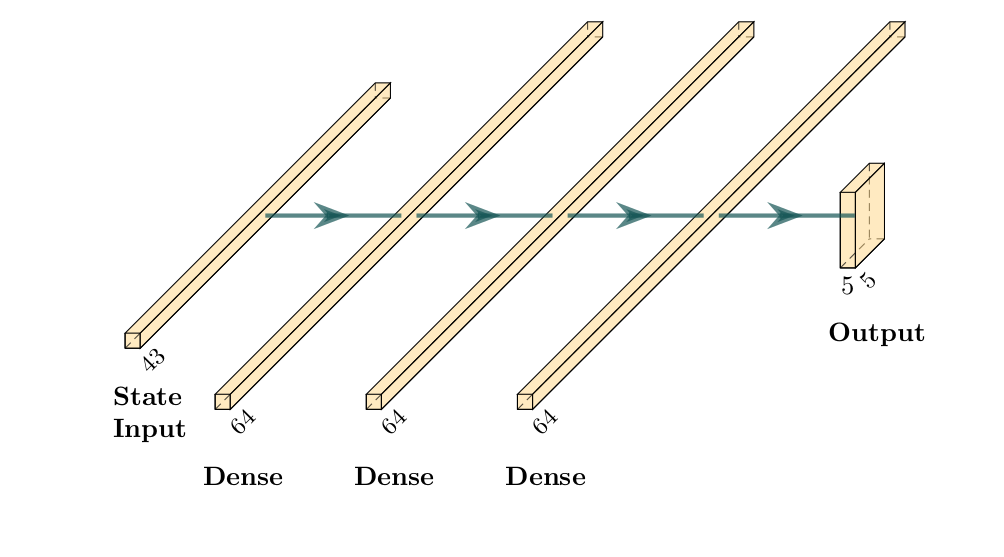
\includegraphics[width=0.5\linewidth]{images/diagrams/contact-network-architecture.png}
  \caption{Footstep evaluation neural network architecture.}
  \label{fig:diagram-contactnet-architecture}
\end{figure}

%%%%%%%%%%%%%%%%%%%%%%%%%%%%%%%%%%%%%%%%%%%%%%%%%%%%%%%%%%%%%%%%%%%%%%%%%%%%%%%%
\subsection{Training}
\label{subsec:methodology-contactnet-training}

The footstep evaluation network is trained to predict heuristic
footstep cost maps, as described in \cite{bratta_contactnet_2024}.
Training data is generated using the simulation environment outlined
in \autoref{sec:methodology-simulation-environment}, but with planar
terrain. As in \cite{bratta_contactnet_2024}, planar terrain is
sufficient for data collection because the cost maps are masked based
on terrain after inference (see
\autoref{subsec:methodology-contactnet-post-processing}).

During training, 100 robots are simulated in parallel, divided into
four groups of 25. Each group tests a grid of footstep positions for
one foot at a time; the front-left group is illustrated in
\autoref{fig:figure-training-fl-sweep}. An \textit{iteration} is
considered complete once all robots have either successfully
completed or failed their assigned motions. Importantly, all robots
begin each iteration from the same initial state.

\begin{figure}[H]
  \centering
  \includegraphics[width=0.5\textwidth]{images/figures/training-fl-sweep.png}
  \caption{Snapshot showing 25 robots testing different footstep
    positions in parallel. For real data generation, 100 are run in
  parallel, testing 25 footstep positions for each foot at a time.}
  \label{fig:figure-training-fl-sweep}
\end{figure}

Data collection proceeds by chaining multiple iterations together,
with control inputs periodically re-sampled from  $\mathbf u \in
(-0.2, 0.2) \times (-0.2, 0.2) \times (-0.4, 0.4)$ with "$\times$"
being the cartesian product.  After each iteration, the top 10
actions are inserted into a tree structure as edges, with the
resulting state as the leaf node. The tree is explored by randomly
selecting leaves for expansion, and this process continues until a
predefined maximum number of iterations is reached. To ensure data
quality, iterations in which more than 50\% of the robots fall are
discarded, along with their two parent nodes in the tree. This
approach promotes the collection of diverse, yet successful, training
data. This implementation differs in the specifics to
\cite{bratta_contactnet_2024}, while still remaining faithful
to the overall methodology.

\autoref{fig:data-cn-training-distribution} illustrates the
distribution of foot positions in the training dataset. Darker
regions correspond to discrete points on the $5 \times 5$ footstep
grids; a foot occupies a given position if it was moved there in that iteration.

\begin{figure}[H]
  \centering
  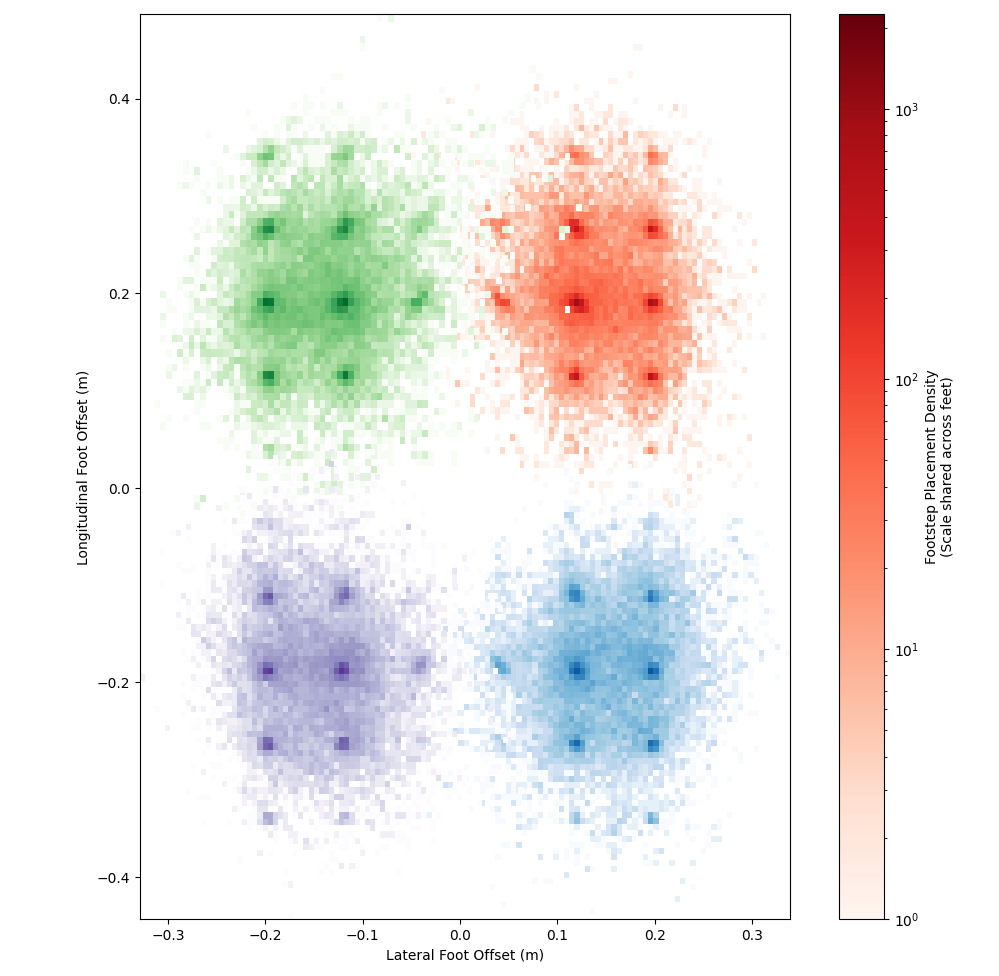
\includegraphics[width=0.5\textwidth]{images/data/foot-placement-heatmaps.png}
  \caption{Foot placement heatmaps showing distribution of foot
    positions in the GaitNet training data. Note that the histograms
  are overlaid in some places, obscuring data underneath.}
  \label{fig:data-cn-training-distribution}
\end{figure}

The purpose of this data collection is to assign a cost to each
potential footstep, forming the candidate set $\mathbf{f_c}$. Costs
are computed heuristically based on simulation outcomes, balancing
stability and efficiency. While similar to the approach in
\cite{bratta_contactnet_2024}, our heuristic differs in several
aspects to better suit the output for the footstep candidate sampling.
\autoref{fig:data-costmap-composition-elements} shows the individual
factors used to construct the footstep candidate maps, and
\autoref{fig:data-costmap-composition-combined} displays the
resulting combined cost map. These factors are described below:

\begin{itemize}
  \item \textit{lin\_vel\_z\_l2}\textemdash Penalizes high vertical
    velocity of the trunk.
  \item \textit{ang\_vel\_xy\_l2}\textemdash Penalizes high angular
    velocity of the trunk in     the horizontal axes.
  \item \textit{joint\_torques\_l2}\textemdash Penalizes high joint torques.
  \item \textit{joint\_acc\_l2}\textemdash Penalizes high joint accelerations.
  \item \textit{control\_error}\textemdash Penalizes errors between the control
    input and actual robot motion.
  \item \textit{inscribed\_circle\_radius}\textemdash Measures the distance
    from the COM to the nearest edge of the support polygon. This
    encourages the robot to keep its COM in a stable position.
  \item \textit{foot\_hip\_distance}\textemdash Measures the distance
    between the hip and foot in the $XY$ plane. This encourages the
    robot to keep its feet moving along with the body.
\end{itemize}

\begin{figure}[H]
  \centering
  \begin{subfigure}[T]{0.65\textwidth}
    \centering
    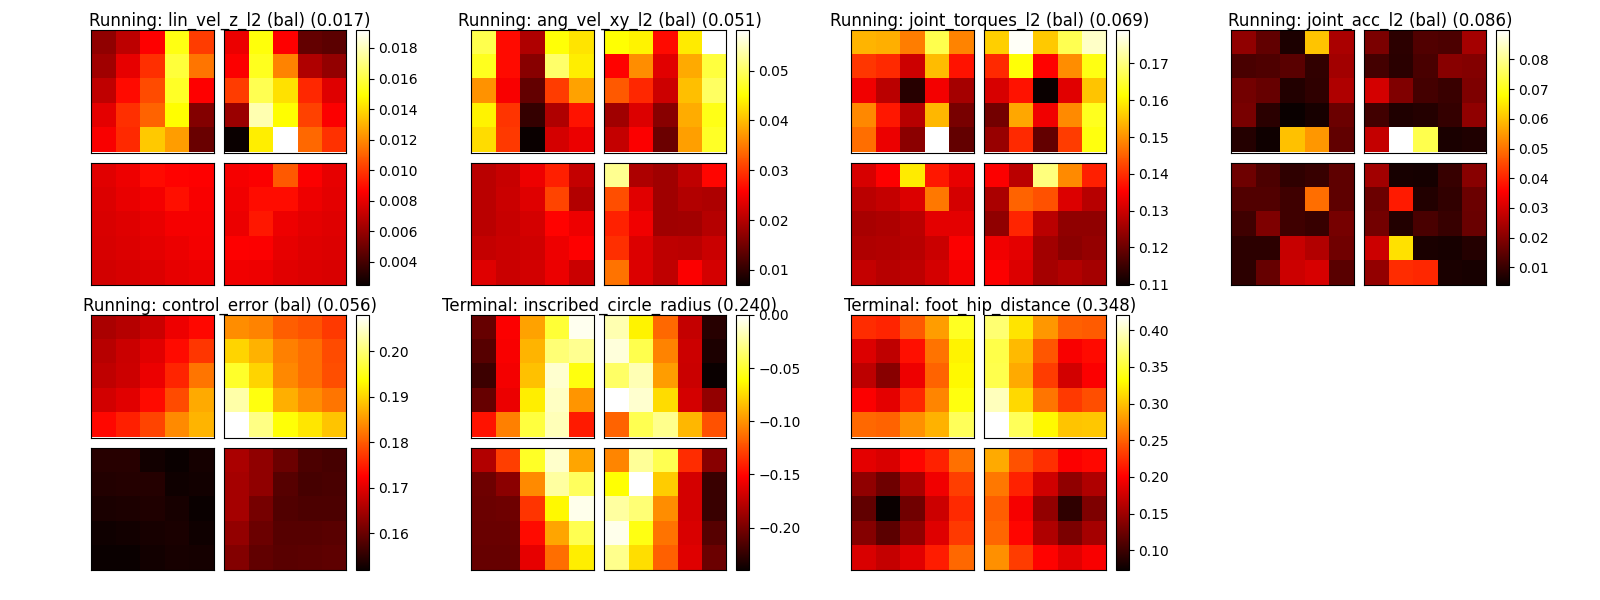
\includegraphics[width=\textwidth]{images/data/training/costmap-composition/elements.png}
    \caption{Factors influencing footstep candidate maps. \textit{(bal)}
      indicates that the values for each leg were balanced to have a
      lower spread, mitigating factors that consistently prefer one leg
      over another. The last number in parenthesis indicates the total
    range of the data, the most important factor for the combined cost map.}
    \label{fig:data-costmap-composition-elements}
  \end{subfigure}
  \hfill
  \begin{subfigure}[T]{0.3\textwidth}
    \centering
    \includegraphics[width=\textwidth]{images/data/training/costmap-composition/combined.png}
    \caption{Combined cost map from factors in (a) (not normalized).}
    \label{fig:data-costmap-composition-combined}
  \end{subfigure}
  \hfill
  \caption{Footstep candidate map composition. (a) shows the individual
    factors that make up the footstep candidate maps, while (b) shows
  the   combined cost map.}
  \label{fig:data-costmap-composition}
\end{figure}

As in \cite{bratta_contactnet_2024}, the cost maps are normalized to
enhance training performance. Our approach differs in that the maps
are normalized directly to the range $[0, 1]$, rather than preserving
only the relative ordering of costs as in
\cite{bratta_contactnet_2024}. This direct normalization is crucial
for providing the upstream GaitNet model with maximal information.

%%%%%%%%%%%%%%%%%%%%%%%%%%%%%%%%%%%%%%%%%%%%%%%%%%%%%%%%%%%%%%%%%%%%%%%%%%%%%%%%
\subsection{Post-Processing}
\label{subsec:methodology-contactnet-post-processing}

The primary purpose of the footstep evaluation network is to provide
high-quality footstep candidates to the GaitNet model.
\autoref{fig:diagram-costmap-processing} illustrates the processing pipeline.

The raw cost map output from the footstep evaluation network
(\autoref{fig:diagram-costmap-processing-raw}) is first upsampled
(\autoref{fig:diagram-costmap-processing-upsample}) to increase the
resolution of possible footstep positions and to match the resolution
of the terrain data. Next, noise is added
(\autoref{fig:diagram-costmap-processing-noise}) to encourage
exploration of a more diverse set of footstep positions; without this
noise, all candidates would cluster in close proximity.

\begin{todo}
  update the number of candidates in text and diagram
\end{todo}

The cost map is then filtered based on the robot state and terrain
data (\autoref{fig:diagram-costmap-processing-cspace}) to mask out
invalid actions. This includes positions that are too close to
terrain edges and movements that would attempt to reposition a leg
already in the swing phase (as illustrated by the Front Right leg in
the figure). Additional masking occurs based on the total number of
legs in the swing phase; when 2 legs are already in swing, all
remaining options are masked out to prevent unstable motions.
Finally, the top 8 candidates from each leg are selected
(\autoref{fig:diagram-costmap-processing-topk}) for processing by
GaitNet. If fewer than 8 valid candidates exist for a given leg,
no-action candidates are added to maintain consistent tensor dimensions.

% === Define layout constants ===
\def\imgwidth{0.16\textwidth}
\def\xgap{2em}          % horizontal gap between images
\def\arrowwidth{1.2em}  % controls arrow length
\def\arrowshift{0.5em} % vertical offset of arrows

\begin{figure}[H]
  \centering
  \begin{tikzpicture}[node distance=\xgap, baseline=(current bounding
    box.center)]

    % === Style for image blocks ===
    \tikzset{
    imgblock/.style={inner sep=0pt, outer sep=0pt, align=center}     }

    % === Subfigure nodes ===
    \node[imgblock] (a)
    {\subcaptionbox{Raw\label{fig:diagram-costmap-processing-raw}}
    {\includegraphics[width=\imgwidth]{images/diagrams/cost-map-processing/1-default.png}}};

    \node[imgblock, right=of a]
    (b)
    {\subcaptionbox{Upsample\label{fig:diagram-costmap-processing-upsample}}
    {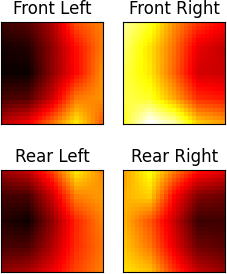
\includegraphics[width=\imgwidth]{images/diagrams/cost-map-processing/2-upscale.png}}};

    \node[imgblock, right=of b]
    (c)
    {\subcaptionbox{Noise\label{fig:diagram-costmap-processing-noise}}
    {\includegraphics[width=\imgwidth]{images/diagrams/cost-map-processing/3-noise.png}}};

    \node[imgblock, right=of c]
    (d)
    {\subcaptionbox{C-space\label{fig:diagram-costmap-processing-cspace}}
    {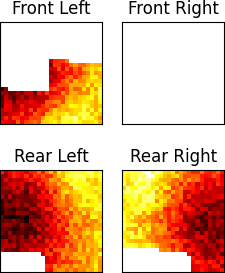
\includegraphics[width=\imgwidth]{images/diagrams/cost-map-processing/4-masked.png}}};

    \node[imgblock, right=of d]
    (e)     {\subcaptionbox{TopK
      (green)\label{fig:diagram-costmap-processing-topk}}
    {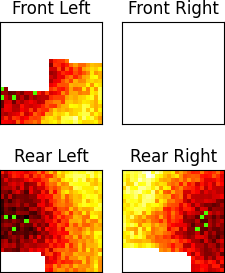
\includegraphics[width=\imgwidth]{images/diagrams/cost-map-processing/5-selected.png}}};

    % === Arrows ===
    \foreach \src/\dst in {a/b, b/c, c/d, d/e}{
      \draw[->, thick] ([yshift=\arrowshift]\src.east) --
    ++(\arrowwidth,0) --       ([yshift=\arrowshift]\dst.west);     }

  \end{tikzpicture}

  \caption{Cost map processing pipeline. Shows how the raw cost map
  is processed to produce the final footstep candidates.}
  \label{fig:diagram-costmap-processing}
\end{figure}
